\documentclass[a4paper,14pt]{article}
\usepackage[a4paper, mag=1000, left=2.5cm, right=1cm, top=2cm, bottom=2cm, headsep=0.7cm, footskip=1cm]{geometry}
\usepackage[utf8]{inputenc}
\usepackage[T2A]{fontenc}
\usepackage[english,russian]{babel}
\usepackage{indentfirst}
%\usepackage[dvipsnames]{xcolor}
\usepackage[colorlinks]{hyperref}
\usepackage{amsfonts} 
\usepackage{amsmath}
\usepackage{amssymb}
\usepackage{graphicx}
\usepackage{float}

\DeclareGraphicsExtensions{.png,.jpg}

\usepackage{fancyhdr}
\pagestyle{fancy}
\fancyhead[LE,RO]{\thepage}
\fancyfoot{}

\usepackage{listings}

\hypersetup{linkcolor=black}

\title{non-linear equations}
\author{Крылова Екатерина}
\date{2024}
\thispagestyle{empty}
\begin{document}
	
	\begin{titlepage}
		\begin{center}
			\textsc{
				Санкт-Петербургский политехнический университет имени Петра Великого \\[5mm]
				Физико-механический институт\\[2mm]
				Высшая школа прикладной математики и физики            
			}   
			\vfill
			\textbf{\large
				Интервальный анализ\\
				Отчёт по лабораторной работе №4 \\[3mm]
			}                
		\end{center}
		
		\vfill
		\hfill
		\begin{minipage}{0.5\textwidth}
			Выполнил: \\[2mm]   
			Студент: Крылова Екатерина \\
			Группа: 5030102/10201\\
		\end{minipage}
		
		\hfill
		\begin{minipage}{0.5\textwidth}
			Принял: \\[2mm]
			к. ф.-м. н., доцент \\   
			Баженов Александр Николаевич
		\end{minipage}
		
		\vfill
		\begin{center}
			Санкт-Петербург \\2025 г.
		\end{center}
	\end{titlepage}
	
	\tableofcontents
	\newpage

  \section{Постановка задачи}

  Определить параметры линейной регрессии

  \begin{equation} \label{eq:islau}
    \mathbf{y} = \beta_0 + \beta_1 \mathbf{x},
  \end{equation}

  где \( \mathbf{x} \) --- входные данные, \( \mathbf{y} \) --- интервальные
  выходные данные, \( \beta_0 \), \( \beta_1 \) --- параметры линейной
  регрессии.

  Для калибровки измерителя, на вход подаётся набор постоянных
  напряжений

  \begin{equation}
    X = \{ x_i \}.
  \end{equation}

  Для надёжности, для каждого значения \( x \) проводится 100 измерений.

  Получается набор интервальных выборок

  \begin{equation}
    \mathbf{Y} = \{ \mathbf{y}_k \}_{k=1}^{100}.
  \end{equation}

  \( \text{rad}~\mathbf{y} = \frac{1}{2^N} \) В, \( N = 14 \).

  Связь кодов данных и В:

  \begin{equation}
    V = \text{Code} / 16384 - 0.5.
  \end{equation}
  Требуется:
  \begin{enumerate}
    \item   Сделать оценки значений \( \mathbf{Y} \) двумя способами:

    \begin{itemize}
      \item in: как интервал между первым и третьим квартилем
      \item ex: как границы бокс-плота
    \end{itemize}
  
    \item Решить ИСЛАУ (\ref{eq:islau}) для внутренних и внешних оценок
    \( \mathbf{y} \)
  
    \item Построить множество решений \( \beta_0 \), \( \beta_1 \).
  
    \item Построить коридор совместных зависимостей.
  \end{enumerate}
  \section{Теория}

  \subsection{Интервальная мода}

  Имеется интервальная выборка

  \[
    \mathbf{X} = \{ \mathbf{x}_i \}.
  \]

  Сформируем массив интервалов \( \mathbf{z} \) из концов интервалов
  \( \mathbf{X} \).

  Для каждого интервала \( \mathbf{z}_i \) вычисляем число \( \mu_i \)
  интервалов из выборки \( \mathbf{X}_i \), включающих \( \mathbf{z}_i \).

  Максимальные \( \mu_i = \max \mu \) достигаются для индексного множества
  \( K \). Тогда можно найти интервальную моду как мультиинтервал

  \begin{equation}
    \text{mode} \mathbf{X} = \bigcup_{k \in K} \mathbf{z}_k.
  \end{equation}

  \section{Реализаця}

  Лабораторная работа выполнена на языке программирования Python. В ходе
  работы были также использованы библиотеки \verb!numpy! и
  \verb!matplotlib!.


  Ссылка на GitHub репозиторий:
  \url{https://github.com/ekaterinakrylovao/interval-analysis/tree/master/lab4}

  \subsection{Алгоритм}
  Алгоритм поиска оценок параметров линейной регрессии заключается в следующем.

  Каждый из файлов содержит 100 фреймов, каждый из которых включает
  1024 массива, состоящих из 8 двухбайтовых значений. В результате
  обработки этих данных было сформировано \( 1024 \times 8 = 8192 \)
  интервальных систем линейных алгебраических уравнений: 

  \[
    \begin{pmatrix}
    [x_1 - \text{rad} \mathbf{y}, x_1 + \text{rad} \mathbf{y}] &
    [1 - \text{rad} \mathbf{y}, 1 + \text{rad} \mathbf{y}] \\
    \vdots & \vdots \\
    [x_8 - \text{rad} \mathbf{y}, x_8 + \text{rad} \mathbf{y}] &
    [1 - \text{rad} \mathbf{y}, 1 + \text{rad} \mathbf{y}]
    \end{pmatrix}
    \begin{pmatrix}
    \beta_1 \\
    \beta_0
    \end{pmatrix}
    = \begin{pmatrix}
    \hat{\mathbf{y}}_{1i} \\
    \vdots \\
    \hat{\mathbf{y}}_{8i}
    \end{pmatrix}, \ i \in \overline{1,8192}
  \]

  Для каждого отдельного пикселя фрейма:
  \begin{itemize}
    \item \( x_j \) --- вольтаж, определяемый по названию файла
    \item \( \hat{\mathbf{y}}_{ji} \) --- оценка значения, соответствующее каждому пикселю (по каждому фрейму)
    \item \( j \) --- порядковый номер файла
    \item  \( i \) --- номер пикселя внутри файла
    \item \( \beta_0 \) и \( \beta_1 \) --- параметры линейной регрессии
  \end{itemize}

  Полчуенные множества интервальных оценок:
  \begin{itemize}
    \item \( \mathbf{B}_0 = \{ \mathbf{\beta}_0 \}_{i=1}^{8192} \)
    \item \( \mathbf{B}_1 = \{ \mathbf{\beta}_1 \}_{i=1}^{8192} \)
  \end{itemize}

  Оценка каждого
  из параметров линейной регрессии производится следующим образом:

  \[ \hat{\mathbf{\beta}}_0 = \text{mode} \mathbf{B}_0, \]
  \[ \hat{\mathbf{\beta}}_1 = \text{mode} \mathbf{B}_1. \]

  Таким образом, конечные значения \( \hat{\mathbf{\beta}}_0 \) и
  \( \hat{\mathbf{\beta}}_1 \) служат наиболее вероятными оценками
  параметров регрессии, что позволяет более точно анализировать
  зависимость между переменными в исследуемых данных.

  \section{Результаты}

  \subsection{Внутренняя оценка}

  Результаты внутренней оценки

  \[
    \text{mode} \mathbf{B}_0
      = \{ [8083.32, 8083.33], [8086.78, 8086.8] \},
  \]
  \[
    \text{mode} \mathbf{B}_1 = [13074.2, 13074.5].
  \]

    \begin{figure}[H]
        \begin{center}
            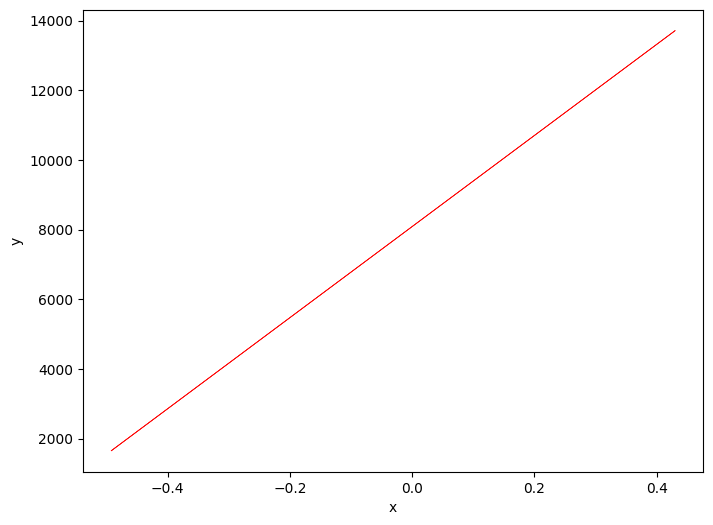
\includegraphics[width = 0.65\textwidth]{mode_in}
            \caption{Коридор совместных зависимостей для внутренней оценки.}
    \label{figure:int_est}
        \end{center}
    \end{figure}

  \subsection{Внешняя оценка}

  Результаты внешней оценки

  \[
    \text{mode} \mathbf{B}_0 = \bigcap_{i=1}^{8192} \mathbf{\beta}_{0i}
      = [7928.86, 8223.23],
  \]
  \[
    \text{mode} \mathbf{B}_1 = \bigcap_{i=1}^{8192} \mathbf{\beta}_{1i}
      = [13101.8, 13570.1].
  \]

    \begin{figure}[H]
        \begin{center}
            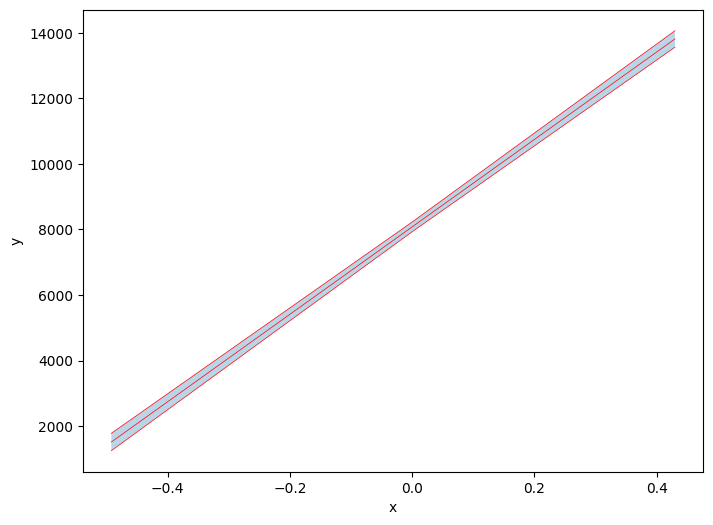
\includegraphics[width = 0.65\textwidth]{mode_ex}
            \caption{Коридор совместных зависимостей для внешней оценки.}
    \label{figure:ext_est}
        \end{center}
    \end{figure}

    \clearpage
    \section{Выводы}
    В ходе выполнения лабораторной работы была реализована методика оценки  
    параметров линейной регрессии на основе интервальных данных. 

    Что удалось сделать:
    
    \begin{itemize}  
      \item Разработать алгоритм для вычисления внутренних и внешних границ  
        оценок параметров линейной регрессии для учёта  
        неопределённости исходных данных.  
      \item Получить интервальные значения параметров \( \beta_0 \) и  
        \( \beta_1 \), которые отражают возможный диапазон их изменения.  
      \item Построить области совместной зависимости, визуализирующие  
        интервальные решения и позволяющие анализировать устойчивость модели.  
    \end{itemize}  
    
    Полученные результаты демонстрируют, что данный подход обеспечивает более  
    адекватное моделирование зависимостей в условиях неопределённости данных.  
    Методика особенно полезна в ситуациях, где точность измерений  
    варьируется, и требуется надёжная оценка параметров модели.  
  \end{document}
